\section{Floquetifying the $\mathbf{\qcode{4, 2, 2}}$ code}\label{sec:floquetifying_422}

Let's warm up with one of the simplest interesting codes around: the $\qcode{4, 2, 2}$ code.
This is a stabilizer code, which we'll define as
$\MMM = [\langle Z_1 Z_2 Z_3 Z_4 \rangle, \langle X_1 X_2 X_3 X_4 \rangle]$.
The aim of this section is to prove the following:
\begin{theorem}\label{thm:4_2_2_double_hexagon_equivalence}
The $\qcode{4, 2, 2}$ stabilizer code is equivalent as a ZX-diagram to a $\qcode{12, 2, 2}$ Floquet code with period 6,
which we call the \textbf{double hexagon code}.
\end{theorem}
In \Cref{fig:4_2_2_rewritten}, we show three equivalent ZX-diagrams depicting seven timesteps of this code.
Here the grey squares, grey numbers, wire colours and wire styles (solid/dashed) have no meaning in the ZX-calculus;
they're just visual aids.
The grey squares denote timesteps of the $\qcode{4, 2, 2}$ code, and the grey numbers and coloured/styled lines will be explained shortly.
The leftmost diagram is the most natural one;
it shows measurements of $Z_1 Z_2 Z_3 Z_4$ and $X_1 X_2 X_3 X_4$ alternating at each timestep.
The second diagram is obtained from the first by unfusing every spider in the center of a grey square into two spiders,
and unfusing every spider in the corner of a grey square into three spiders.
The third is identical to the second in the ZX-calculus - all we've done is coloured and styled certain wires,
and labelled all one-legged spiders and black wires with an integer.
Now, in the leftmost diagram,
we interpret the four vertical lines as the world-lines of the four qubits of the code.
But we need not do this!
The ZX-diagram remains equivalent if we choose to interpret different wires as qubit world-lines.
This is exactly what the colours and styles in the rightmost diagram are for;
each colour-style pair denotes a different qubit world-line.
Since there are twelve world-lines, we're now viewing this as a system of twelve qubits, rather than four.
\begin{figure}[t]
    \centering
    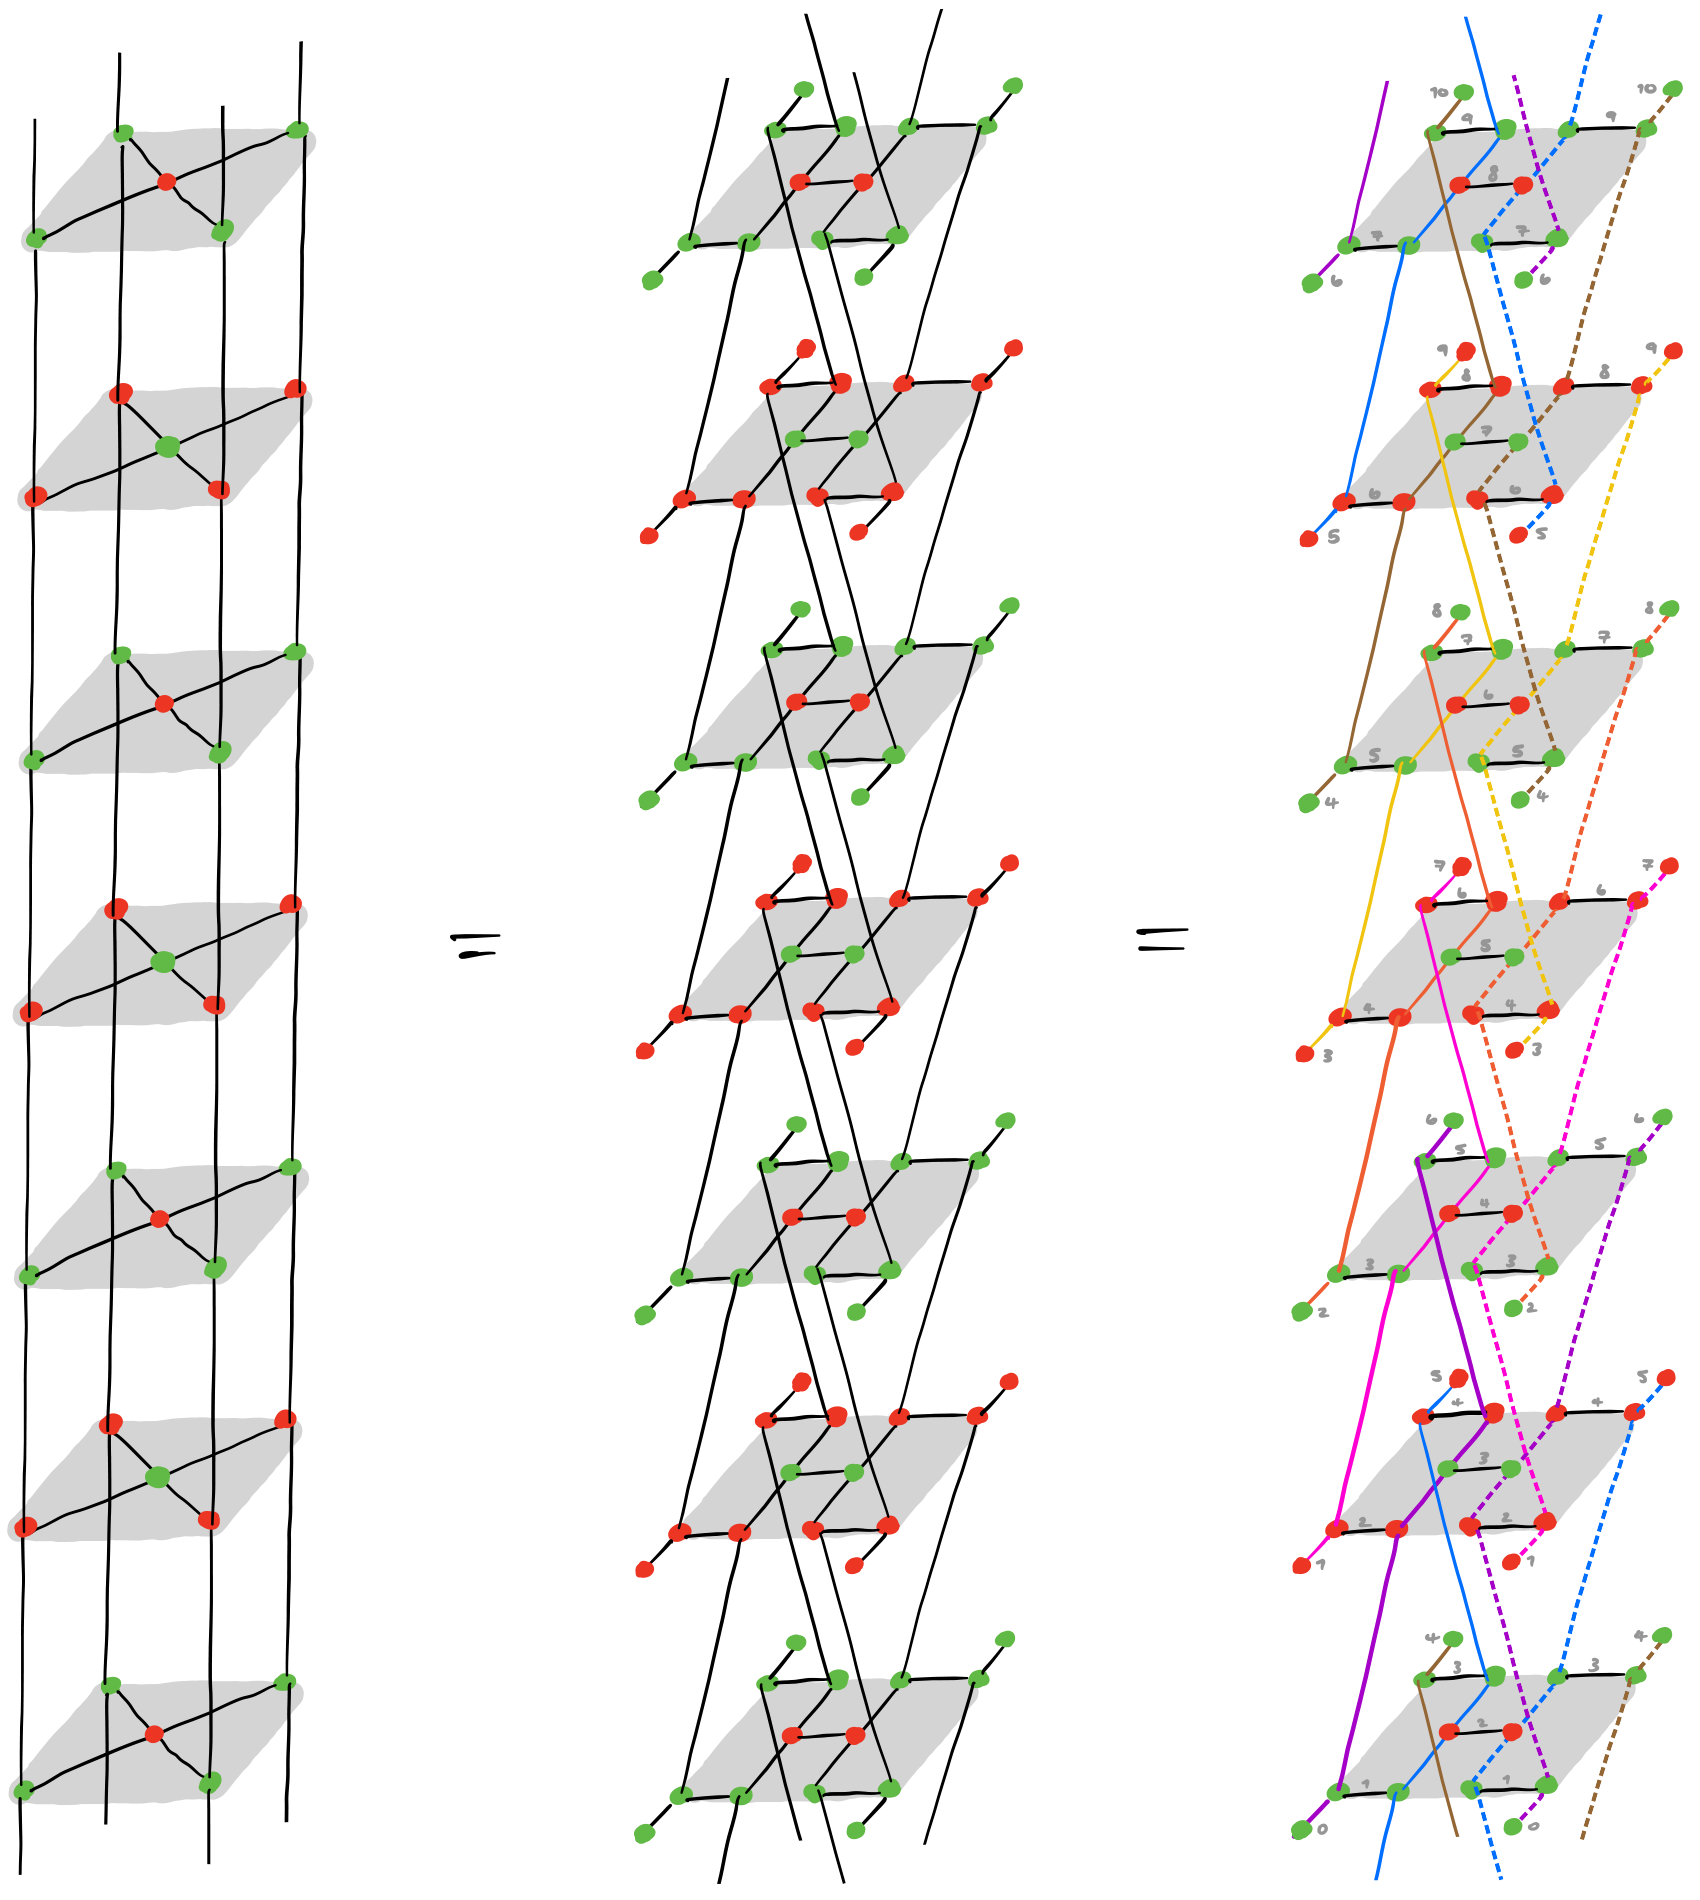
\includegraphics[width=340pt]{figures/floquetifying/422/zx_rewritten}
    \caption{Three equivalent ZX-diagrams for seven timesteps of the $\qcode{4, 2, 2}$ code.}
    \label{fig:4_2_2_rewritten}
\end{figure}

Let's make some observations about this rightmost diagram.
Firstly, if we follow the world-line of any particular qubit up the page,
the integer labels incident to it form an increasing sequence.
For example, starting from the bottom of the diagram and following the solid purple qubit upwards,
the integers incident to it form the sequence $[0, 1, \ldots, 6]$.
We can thus think of these integers as a new set of timesteps for this diagram.
Next, notice that we can interpret all the uncoloured black wires like
\ 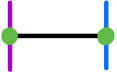
\includegraphics[height=1\baselineskip, valign=c]{figures/floquetifying/zx_calculus/ZZ}
\ and
\ 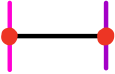
\includegraphics[height=1\baselineskip, valign=c]{figures/floquetifying/zx_calculus/XX}
\ as weight two $Z_u Z_v$ and $X_u X_v$ measurements (respectively) between qubits.
Furthermore, the qubit world-lines only have limited interactions with each other via these measurements.
Specifically, if we define ordered lists
$\mathbf{colours} = [
\mathbf{purple}, ~
\mathbf{pink}, ~
\mathbf{orange}, ~
\mathbf{yellow}, ~
\mathbf{brown}, ~
\mathbf{blue}]$
and
$\mathbf{styles} = [
\mathbf{solid}, ~
\mathbf{dashed}]$,
and let qubit $(i, j)$ denote the qubit with the $i$-th colour and $j$-th style,
where $i$ and $j$ are taken modulo 6 and 2 respectively,
then looking closely we see that qubit $(i, j)$ is only ever involved in
a measurement with the three qubits $(i+1, j), (i-1, j)$ and $(i, j+1)$.
So supposing we now wanted to lay out these qubits on a planar 2D chip,
a natural geometry would be a `double hexagon', as in the rightmost diagram of \Cref{fig:detector_4_2_2_double_hexagon}.

In fact, recalling the diagrammatic equation\
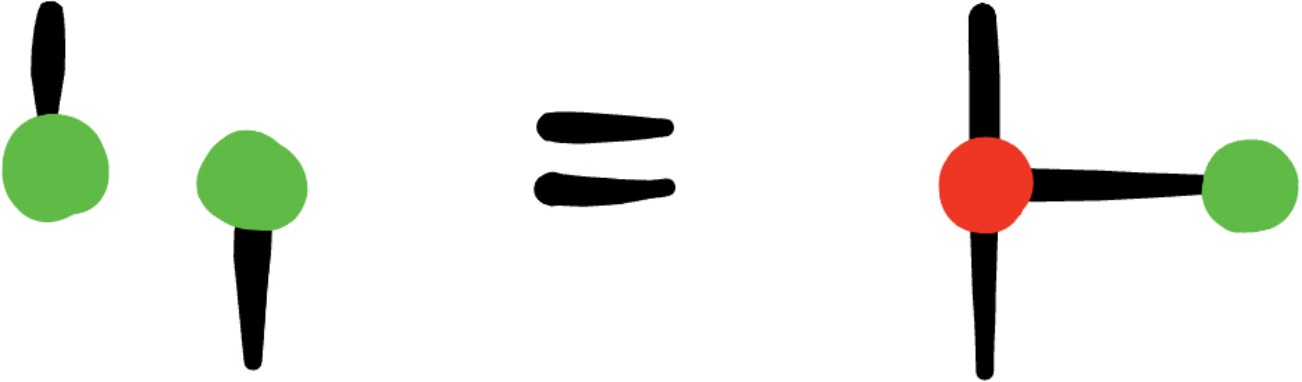
\includegraphics[height=1.1\baselineskip, valign=c]{figures/floquetifying/zx_calculus/single_qubit_measurement_splits}\ ,
which says non-destructive single qubit Pauli measurements disconnect wires,
we can also interpret all one-legged spiders as one half of such a measurement.
This interpretation is valid,
in that the timestep at which the world-line of qubit $(i, j)$ `ends' at a one-legged spider
is the same as the timestep at which it `resumes' via another one-legged spider further up the page.
Finally, we can see that this pattern of colours and styles repeats itself every six timesteps.

\begin{figure}[b]
    \centering
    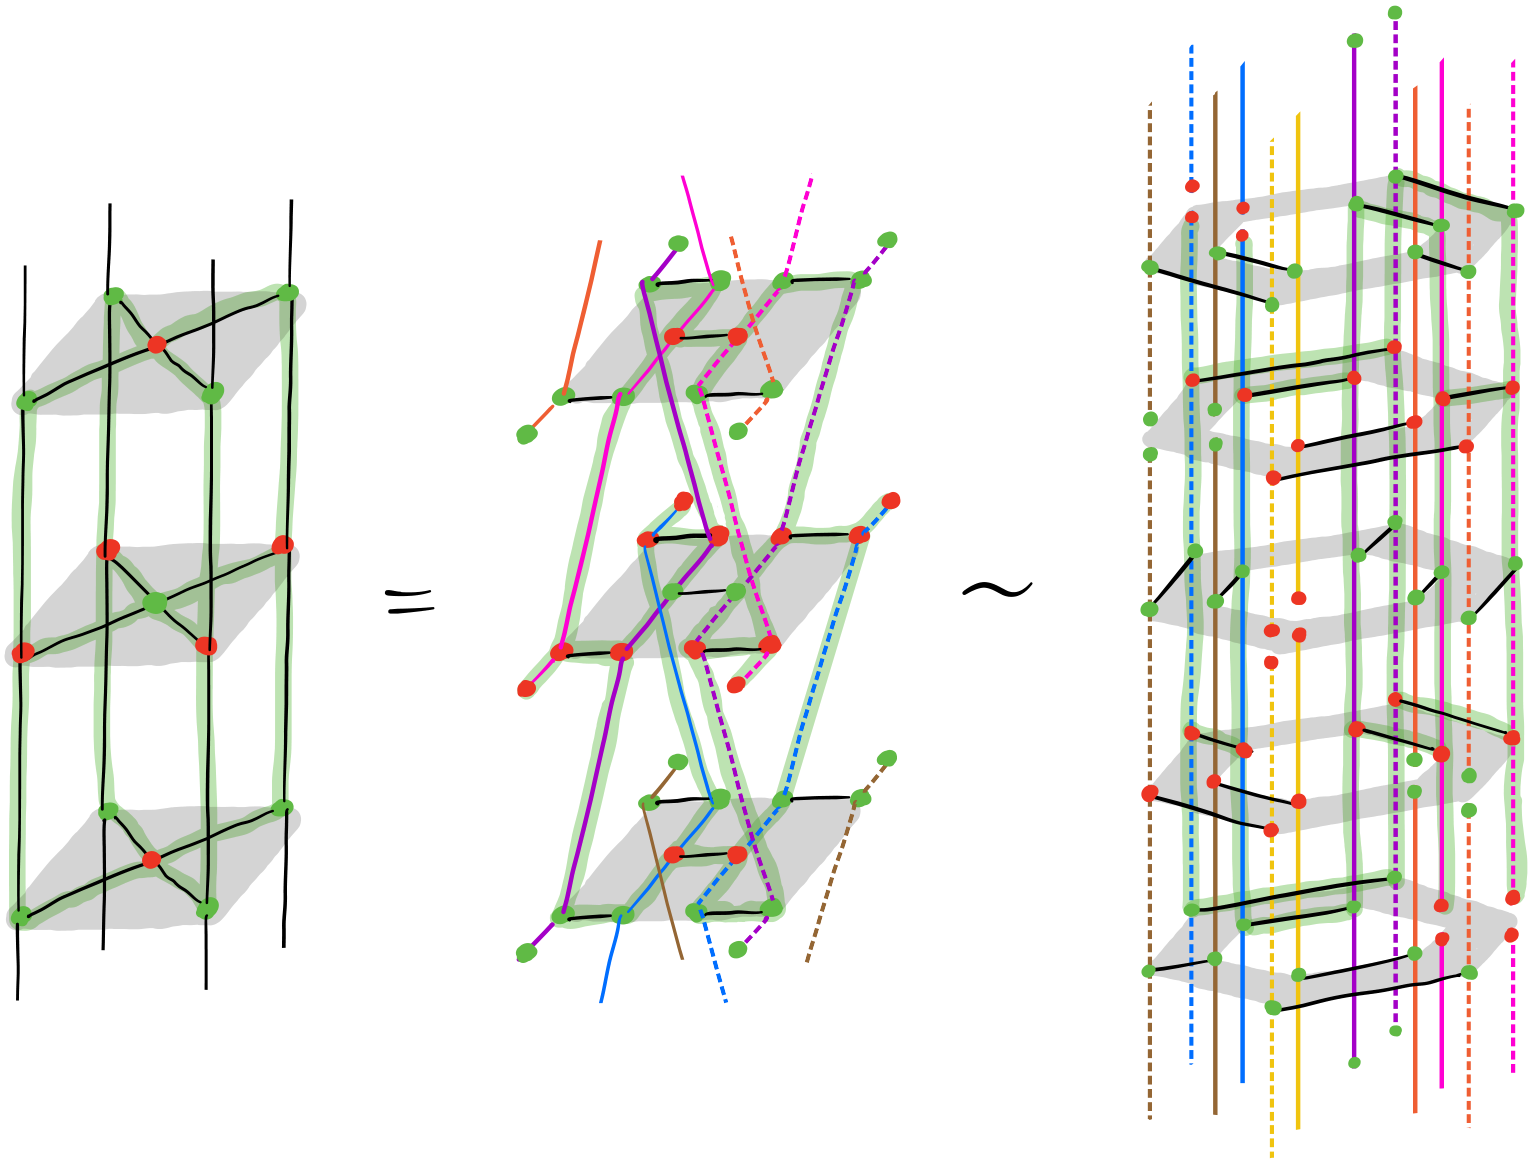
\includegraphics[width=330pt]{figures/floquetifying/422/floquetified/detector}
    \caption{
        A detecting region in the $\qcode{4, 2, 2}$ code and its image in the double hexagon code.
        We use the ($\sim$) symbol between the second and third diagrams rather than an equals sign because,
        although the two codes can be viewed as having equivalent ZX-diagrams,
        these two particular subdiagrams are not equivalent -
        the rightmost one has more input and output wires, for example.}
    \label{fig:detector_4_2_2_double_hexagon}
\end{figure}

From this analysis, we can now interpret the rightmost ZX-diagram as an ISG code;
we can write down the measurements that each qubit undergoes at each timestep,
and consequently we can define the measurement schedule described by this diagram.
We get $\MMM = [\MMM_0, \ldots, \MMM_5]$, where:
\begin{equation}\label{eq:floquetified_4_2_2_measurement_schedule}
\MMM_t = \stretchleftright[1000]
{<}
{\begin{array}{c}
     X_{(t, 0)}, \\
     X_{(t, 1)}, \\
     X_{(t+1, 0)}X_{(t+2, 0)}, \\
     X_{(t+1, 1)}X_{(t+2, 1)}, \\
     X_{(t+3, 0)}X_{(t+3, 1)}, \\
     X_{(t+4, 0)}X_{(t+5, 0)}, \\
     X_{(t+4, 1)}X_{(t+5, 1)} \\
\end{array}}
{>}
\text{~~if $t$ even,}
\qquad\qquad
\MMM_t = \stretchleftright[1000]
{<}
{\begin{array}{c}
     Z_{(t, 0)}, \\
     Z_{(t, 1)}, \\
     Z_{(t+1, 0)}Z_{(t+2, 0)}, \\
     Z_{(t+1, 1)}Z_{(t+2, 1)}, \\
     Z_{(t+3, 0)}Z_{(t+3, 1)}, \\
     Z_{(t+4, 0)}Z_{(t+5, 0)}, \\
     Z_{(t+4, 1)}Z_{(t+5, 1)} \\
\end{array}}
{>}
\text{~~if $t$ odd.}
\end{equation}
One can then calculate the group $\isg{t}$, and consequently $\lpg{t}$.
It turns out $\isg{t}$ is established whenever $t \geq T = 3$,
and can be minimally generated by the seven generators of $\MMM_t$,
plus three weight-six Paulis $s_{t-1}, s_{t-2}$ and $s_{t-3}$, where:
\begin{equation}\label{eq:floquetified_4_2_2_s_t}
s_t = \begin{cases}
          X_{(t, 0)}X_{(t, 1)}X_{(t-1, 0)}X_{(t-1, 1)}X_{(t-2, 0)}X_{(t-2, 1)} &\text{ if $t$ even} \\
          Z_{(t, 0)}Z_{(t, 1)}Z_{(t-1, 0)}Z_{(t-1, 1)}Z_{(t-2, 0)}Z_{(t-2, 1)} &\text{ if $t$ odd} \\
\end{cases}
\end{equation}

Since we have 10 independent generators on 12 qubits, we can conclude that $\lpg{t} \cong \PPP_2$ for all $t \geq 3$.
This then proves most of \Cref{thm:4_2_2_double_hexagon_equivalence};
namely that the double hexagon code encodes 2 logical qubits and has period 6.
The proof that the distance of the new Floquet code remains two is deferred to \Cref{sec:double_hexagon_code}.

In addition to being able to work with detectors, stabilizers and logical operators algebraically, as above,
the mapping of these objects from the $\qcode{4, 2, 2}$ code to the double hexagon code
can be seen graphically via Pauli webs.
In \Cref{fig:detector_4_2_2_double_hexagon} we show a detecting region in the $\qcode{4, 2, 2}$ code
and its image in the double hexagon code.
From the rightmost diagram of this figure,
and recalling the rules for mapping a detecting region to a detector from \Cref{subsubsec:detectors},
one can see that the corresponding detector in the double hexagon code consists of eight measurements.
Specifically, in the bottom layer, we include two $Z \otimes Z$ measurements between blue and purple qubits,
and two single qubit $Z$ measurements on pink qubits.
In the top layer, we include two $Z \otimes Z$ measurements between purple and pink qubits,
and two single qubit $Z$ measurements on blue qubits.
Since every detecting region in the $\qcode{4, 2, 2}$ code is equivalent to the one on the left of this figure
(up to a space-time translation and exchanging the roles of $Z$ and $X$),
every detecting region in the double hexagon code is equivalent to the one on the right
(again up to a space-time translation and $Z \leftrightarrow X$ interchange).

One could justifiably point out here that we seem to have made things worse;
we've taken a $\qcode{4, 2, 2}$ ISG code and turned it into a $\qcode{12, 2, 2}$ ISG code,
and what's more, each detector now consists of eight measurements rather than two, so would seem to be noisier!
The trade-off is that now every measurement is weight-two or weight-one, rather than weight-four.
As a general rule, the higher the measurement weight, the noisier it will be.
In particular, weight-one and weight-two measurements can be performed natively in some architectures,
whereas higher-weight measurements are implemented via extraction circuits,
which give more opportunities for noise to interfere.

On a higher-level, one can view this Floquetification process as a reinterpretation of the time direction
in a ZX-diagram.
Below, we use two blue prisms (square and hexagonal)
as abstractions of ZX-diagrams for the $\qcode{4, 2, 2}$ code and double hexagon code respectively.
In grey we show how a timeslice in the double hexagon code corresponds to an angled slice of the $\qcode{4, 2, 2}$ code:
\begin{equation}\label{eq:timeslice_4_2_2_double_hexagon}
\begin{aligned}
    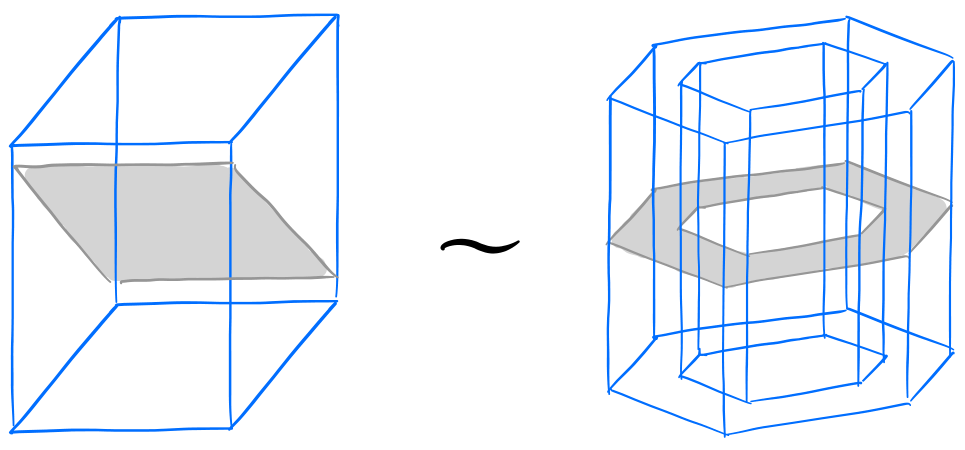
\includegraphics[width=230pt]{figures/floquetifying/422/floquetified/abstract_timeslice}
\end{aligned}
\end{equation}